\subsection{Histoire et anatomie de l'aphasie}

Louis Victor Leborgne, né en 1809 à Moret-sur-Loing commençe à perdre 
la capacité de parler à l'age de 30 ans.
Il est admis à l'hôpital de Bicêtre où il passerait 21 ans pendant lesquelles, 
il ne communique qu'en produisant le son ``tan'', typiquement répété deux fois, 
si bien qu'on lui a donné le surnom ``monsieur Tan tan''~\cite{Mohammed_Narayan_Patra_Nanda_2018}.

Le 11 avril 1861, monsieur Leborgne est examiné par Dr.~Pierre Paul Broca 
pour une gangrène dans son pied droit.
Dr.~Broca s'intéresse au trouble linguistique dont souffre son patient~\cite{Lorch_2011}.
Il fait l'observation que les facultés intellectuelles et motrices de monsieur Leborgne sont intactes,
il en conclut qu'elles ne peuvent être à l'origine de son handicape. 
Dr.~Broca donne le nom ``aphémie'' à ce type de situation~\cite{Broca}, il en écrit :

\begin{quotation}
    ``Cette abolition de la parole, chez des individus qui ne sont ni paralysés ni idiots, constitue un symptôme assez singulier pour qu'il me paraisse utile de la désigner sous un nom spécial. Je lui donnerai donc le nom d'aphémie (\textgreek{a} privatif ; \textgreek{fhmi}, je parle, je prononce) ; car ce qui manque à ces malades, c'est seulement la faculté d'articuler les mots.''
    \begin{flushright}
        \rm --- \barecite{Broca}.
    \end{flushright}
\end{quotation}

Dr.~Broca prend ce constat comme confirmation de ce qu'il appelait 
``le principe de localisations cérébrales''.
Il s'agit de l'idée que le cerveau fonctionne comme système à plusieurs composants plutôt qu'un monolithe
et que les fonctions cognitives sont spatialement localisées~\cite{Fodor_1983}.

Quand monsieur Leborgne est décédé le 17 avril, Dr.~Broca lui fait l'autopsie.
En ouvrant le crâne, il observe une lésion dans le cortex inférieur gauche du lobe frontale 
(voir Figure~\ref{fig.leborgne-brain}).
Il en déduit que 
\begin{enumerate*}[label=(\arabic*)]
    \item cette lésion était à l'origine de l'aphémie de monsieur Leborgne et que 
    \item la partie affectée du cerveau est responsable d'articuler des expressions dans le langage%
    ~\cite{Broca,Lorch_2011,Mohammed_Narayan_Patra_Nanda_2018}.
\end{enumerate*}

\begin{figure}[htb]
    \begin{center}
        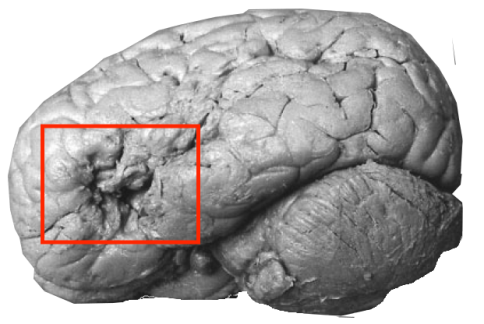
\includegraphics[width=10cm]{assets/images/leborgne-brain.png}
    \end{center}
    \caption[Cerveau de Victor Louis Leborgne avec la lésion encadrée.]
    {Cerveau de Victor Louis Leborgne avec la lésion encadrée~\cite{Lopes_2019}.}
    \label{fig.leborgne-brain}
\end{figure}

Le trouble que Dr.~Broca appelle ``aphémie'' 
est aujourd'hui connu sous le nom d'aphasie de Broca.
Le cas de monsieur Leborgne est largement reconnu comme le premier cas enregistré d'aphasie en général
et d'aphasie de Broca en particulier~\cite{Mohammed_Narayan_Patra_Nanda_2018}.